\documentclass[10pt,letterpaper]{article}
\usepackage[top=0.85in,left=1.0in,right=1.0in,footskip=0.75in]{geometry}

% Use adjustwidth environment to exceed column width (see example table in text)
\usepackage{changepage}

% Use Unicode characters when possible
\usepackage[utf8]{inputenc}

% textcomp package and marvosym package for additional characters
\usepackage{textcomp,marvosym}

% fixltx2e package for \textsubscript
\usepackage{fixltx2e}

% amsmath and amssymb packages, useful for mathematical formulas and symbols
\usepackage{amsmath,amssymb}

% cite package, to clean up citations in the main text. Do not remove.
\usepackage{cite}

% Use nameref to cite supporting information files (see Supporting Information section for more info)
\usepackage{nameref,hyperref}

\usepackage{amsthm}

% line numbers
\usepackage[right]{lineno}

% ligatures disabled
\usepackage{microtype}
\DisableLigatures[f]{encoding = *, family = * }

% rotating package for sideways tables
\usepackage{rotating}

% Remove comment for double spacing
%\usepackage{setspace} 
%\doublespacing

% Text layout
\raggedright
\setlength{\parindent}{0.5cm}
\textwidth 6.25in 
\textheight 8.75in

% Bold the 'Figure #' in the caption and separate it from the title/caption with a period
% Captions will be left justified
\usepackage[aboveskip=1pt,labelfont=bf,labelsep=period,justification=raggedright,singlelinecheck=off]{caption}

% Use the PLoS provided BiBTeX style
\bibliographystyle{plos2015}

% Remove brackets from numbering in List of References
\makeatletter
\renewcommand{\@biblabel}[1]{\quad#1.}
\makeatother

\newtheorem{theorem}{Theorem}
\newtheorem{lemma}{Lemma}
\newtheorem{definition}{Definition}

% Leave date blank
\date{}

% Header and Footer with logo
\usepackage{lastpage,fancyhdr,graphicx}
\usepackage{epstopdf}
\pagestyle{myheadings}
\pagestyle{fancy}
\fancyhf{}

\rfoot{\thepage/\pageref{LastPage}}
\renewcommand{\footrule}{\hrule height 2pt \vspace{2mm}}
\fancyheadoffset[L]{2.25in}
\fancyfootoffset[L]{2.25in}
\lfoot{\sf PLOS}

%% END MACROS SECTION
\begin{document}
\vspace*{0.35in}

\begin{flushleft}
{\Large
\textbf\newline{Descent-based joint optimization}
}
\newline
\\
Jean Feng and Noah Simon
\\

\end{flushleft}
\section*{Abstract}
Tuning regularization parameters in regression problems allows one to control model complexity and induce desired structure. The current method of searching over a $k$-dimensional grid of parameter values is computationally intractable for $k>2$. We propose tuning the penalty parameters by treating it as a continuous optimization problem and updating the parameter values using a descent-based approach. Compared to performing cross validation over a grid, our method is significantly more efficient while achieving the same performance. This descent-based approach enables us to test regularizations with many penalty parameters, through which we discover new regularization methods with superior accuracy. Our experiments are performed on simulated and real data.

\section{Introduction}

Consider the usual regression framework with $p$ features and a response measured on $n$ observations. Let $X$ denote the $n \times p$ design matrix and $y$ the response vector. For ill-posed or high-dimensional problems ($p \gg n$), there can often be an infinite number of solutions that minimize the loss function $L$ but have high generalization error. A common solution is to use regularization, or penalization, to select models with desirable properties, such as smoothness and sparsity.

In recent years, there has been much interest in combining regularization methods to produce models with multiple desired characteristics. Examples include the elastic net (Zou and Hastie 2003), which combines the lasso and ridge penalties, and the sparse group lasso (Simon 2007), which combines the group lasso and lasso penalties. The general form of these regression problems is:

\begin{equation} \label {eq:basic}
\hat f(\lambda_1, ..., \lambda_k) = \arg \min_f L(\boldsymbol{y}, f (\boldsymbol{X})) + \sum\limits_{i=1}^k \lambda_i J_i(f)
\end{equation}
where $L$ is the loss function, $\{J_i\}_{i=1, ..., k}$ are the penalty functions, and $\{\lambda_i\}_{i=1, ..., k}$ are the regularization parameters.

Regularization parameters control the degree of various facets of model complexity (e.g. amount of sparsity or smoothness). Often, the goal is to set the parameters to minimize the fitted model's generalization error. One usually estimates this using a training/validation approach (or cross-validation). There one fits a model on a training set $(X_T, \boldsymbol y_T)$ and measures the model's error on a validation set $(X_V, \boldsymbol y_V)$. The goal then is to choose penalty parameters that minimize the validation error, as formulated in the following optimization problem:
\begin{equation}
\begin{array}{c}
\min_{\boldsymbol{\lambda} \in \Lambda} L(\boldsymbol{y}_V, \hat f (\boldsymbol{X}_V | \boldsymbol{\lambda})) \\
\text{where } \hat f(\cdot | \boldsymbol{\lambda}) = \arg \min_f L(\boldsymbol{y}_T, f (\boldsymbol{X}_T)) + \sum\limits_{i=1}^k \lambda_i J_i(f)
\end{array}
\label{jointopt}
\end{equation}

The simplest approach to solving the problem above is brute force: one fits models over a grid of parameter values and selects the model with the lowest validation error. As long as the grid is large and fine enough, this method of ``grid search" will find a solution close to the global optimum. This approach is the current standard for choosing penalty parameters via train/validation. Unfortunately, it is computationally intractable in cases with more than two parameters. Many variants of grid search have been proposed to increase efficiency, but their runtimes are all exponential in the number of parameters.

In this paper, we propose leveraging the tools of optimization to solve \eqref{jointopt} over the penalty parameter space. We give a gradient descent algorithm for the penalty parameters (to minimize validation error). In contrast to an exhaustive ``grid search'', this ``descent-based'' optimization makes use of the smoothness of our validation-error surface. 

In simulation studies we show that our descent-based optimization produces solutions with the same validation error as those from grid search. In addition, we find that our approach is highly efficient and can solve regressions with hundreds of penalty parameters. Finally, we use this method to analyze regularization methods that were previously computationally intractable. Through this, we discover that a variant of sparse group lasso with many more penalty parameters can significantly decrease error and produce more meaningful models.

Lorbert and Ramadge (2010) presented some related work on this topic. They solved linear regression problems by updating regression coefficients and regularization parameters using cyclical coordinate gradient descent. We take a more general approach that allows us to apply joint optimization to both linear and nonlinear regressions. In particular this paper focuses on three examples that demonstrate the wide applicability of our method: elastic net, sparse group lasso, and additive partial linear models.

In Section 2, we describe descent-based optimization in detail and present an algorithm for solving it in example regressions. In Section 3, we show that our method achieves validation errors as low as those achieved by grid search. In Section 4, we explore variants of the example regression problems that have many more regularization parameters and demonstrate that solving \eqref{jointopt} is still computationally tractable. Finally, we present results on data predicting colitis status from gene expression in Section 5.

\section{Descent-based Joint Optimization}
\subsection{Definition}
Suppose that we have $n$ observations on each of which we have measured $p$ features and a response. Let $\boldsymbol{y}$ be the $n$ response vector and $\boldsymbol{X}$ be the $n \times p$ design matrix. In addition, suppose we are fitting a model $f$ by minimizing a penalized criterion of the form:
\begin{equation}
L(\boldsymbol{y}, f (\boldsymbol{X})) + \sum\limits_{i=1}^k \lambda_i J_i(f)
\end{equation}
where $L$ is the loss function and $(J_i, \lambda_i)$ is the $i$th penalty function and the corresponding penalty parameter.

Suppose we would to select penalty parameters $\boldsymbol{\lambda} = (\lambda_1, ..., \lambda_k)^T$ via a training/validation split. We partition the data into a training set $(\boldsymbol{y}_T , \boldsymbol{X}_T)$ and validation set $(\boldsymbol{y}_V, \boldsymbol{X}_V)$. We choose our penalty parameters to minimize the validation error by solving the following optimization problem:
\begin{equation}
\begin{array}{c}
\arg \min_{\boldsymbol{\lambda} \in \mathbb{R}^k} L(\boldsymbol{y}_V, \hat f(\boldsymbol{X}_V | \boldsymbol{\lambda})) \\
\text{where } \hat f(\cdot | \boldsymbol{\lambda}) = \arg \min_f L(\boldsymbol{y}_T, f (\boldsymbol{X}_T)) + \sum\limits_{i=1}^k \lambda_i J_i(f)
\end{array}
\label{jointopt2}
\end{equation}

For ease of reading, we will use $L_V(\boldsymbol{\lambda})$ to denote $L(\boldsymbol y_V, \hat f(X_V | \boldsymbol{\lambda}))$ since the validation loss is ultimately a function of the penalty parameters.

\eqref{jointopt2} is the explicit, though often unstated, criterion that training/validation methods attempt to minimize to choose penalty parameters . The current standard is to minimize this using an exhaustive grid-search. Grid-based methods solve the joint optimization problem by fitting models over a $k$-dimensional grid $G$ in the penalty parameter space --- the computational runtime of grid-based methods grows exponentially with the number of parameters. While the approach is simple and powerful for a single penalty parameter, optimizing even moderate dimensional functions (3+) via exhaustive grid search is inefficient (and becomes quickly completely intractable).  In addition \eqref{jointopt2} is generally a continuous, piecewise-smooth problem. Using an exhaustive search ignores information available from the smoothness of the surface. 

We propose leveraging the tools of smooth optimization to solve \eqref{jointopt2}. In particular we discuss iterative methods, based on walking in a descent direction until convergence to a local minimum. In the simple case where the criterion is differentiable with respect to the penalty parameters, it is straightforward to use gradient descent or some variant thereof. We show that, with some slight tweaks, gradient descent can be applied in situations where the penalty is only differentiable when restricted to directions involving an active set.

Figure \ref{fig:compare} illustrates the differences between the two approaches. Grid-based method fits a model at every grid point, even though many of these grid points are not close to the global or local minima. We can save significant computational time if we avoid those points unlikely to yield good models. By incorporating information about the shape of the local neighborhood, descent-based methods choose an intelligent descent direction and explore the space more efficiently. 

\begin{figure}
\begin{center}
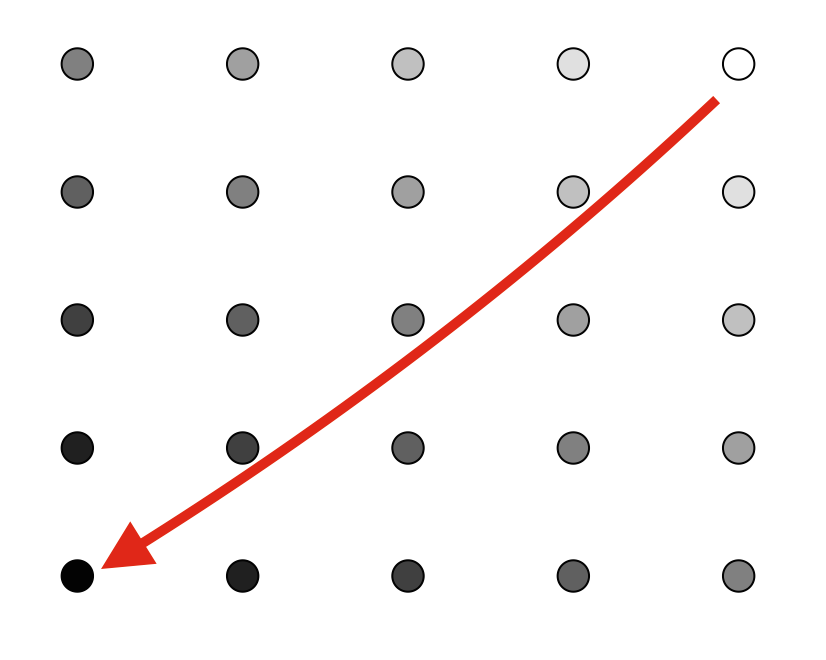
\includegraphics[height=40mm]{grid_search_vs_descent.png}
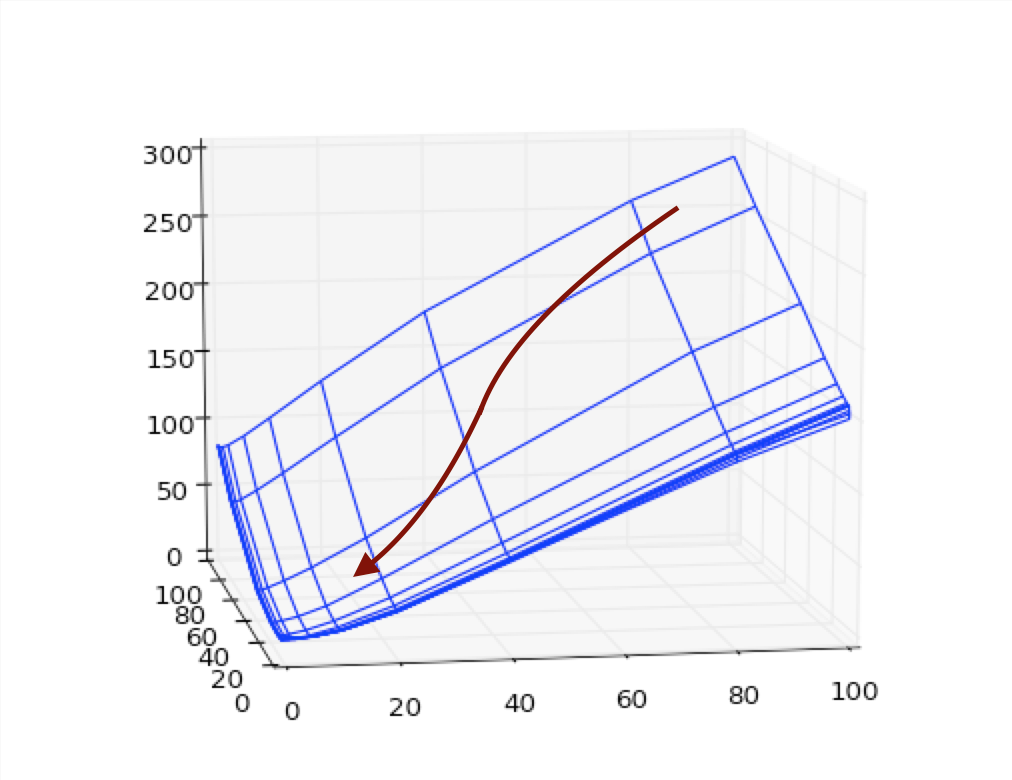
\includegraphics[height=60mm]{surface_in_regularization_parameters.png}
\end{center}
\caption{Left: darker points mean lower validation loss. Descent-based optimization descends in the most direct path towards the point producing the lowest validation loss. Right: The 3D version. We can tune regularization parameters using a grid search... or just descend opposite of the gradient.}
\label{fig:compare}
\end{figure}

Of course, the joint optimization problem is non-convex and therefore our method provides no guarantees. The major benefit of using our method is that it opens up the possibility of using regularization methods that combine multiple penalty terms.

\subsection{Algorithm}

In this section, we describe how to solve joint optimization problems using modified gradient descent. To explain the general idea, we first explain the simple case in which the objective of the joint optimization problem is differentiable.

% In the simple case where the validation loss $L_V(\boldsymbol{\lambda})$ is differentiable, we can directly use gradient descent. If the validation loss is differentiable almost everywhere, such as the lasso and group lasso, we show that we can still solve the problem using a variant of gradient descent. We begin with the simple case to explain the main idea of the algorithm.

\subsubsection{Gradient Descent}

The joint optimization problem is to minimize the validation loss $L(\boldsymbol{y}_V, \hat f(\boldsymbol{X}_V | \boldsymbol{\lambda}))$ by tuning the regularization parameters $\boldsymbol{\lambda}$. In the simplest case, the validation loss is differentiable with respect to $\boldsymbol{\lambda}$, which means that we can simply perform gradient descent. The algorithm is initialized at some point $\boldsymbol{\lambda}^{(0)}$ and at each iteration, we take a step in the direction opposite of the gradient:

\begin{center}
  \fbox{
    \parbox{30em}{
        Choose step size $\alpha$.\\
        Initialize $\boldsymbol{\lambda}^{(0)}$.\\
        For each iteration $k$:
	\begin{equation*}
	\boldsymbol{\lambda}^{(k+1)} := \boldsymbol{\lambda}^{(k)} - \alpha \nabla_{\boldsymbol{\lambda}} L(\boldsymbol{y}_V, \hat f(\boldsymbol{X}_V | \boldsymbol{\lambda}^{(k)}))
	\end{equation*}
	% where $\boldsymbol{g}_V(\boldsymbol{\lambda}^{(k)})$ is any subgradient of $L_V$ at $\boldsymbol{\lambda}^{(k)}$.
	%where $\alpha(\lambda^{(k)})$ is the step size for the $k$th step.
    }
  }
\end{center}
To calculate the gradient, we apply the chain rule:
\begin{equation}
\nabla_{\boldsymbol{\lambda}} L(\boldsymbol{y}_V, \hat f(\boldsymbol{X}_V | \boldsymbol{\lambda})) = \frac{\partial}{\partial \hat f}L_V(\hat f(\boldsymbol{\lambda}))^T \frac{\partial}{\partial \lambda} \hat f(\boldsymbol{\lambda})
\label{chainrule}
\end{equation}
In most joint optimization problems, calculating the first term $\frac{\partial}{\partial \hat f}L_V(\hat f(\boldsymbol{\lambda}))$ is straightforward. To get the second term, recall that $\hat f$ is defined as the model that minimizes
\begin{equation}
L(\boldsymbol{y}_T, f (\boldsymbol{X}_T)) + \sum\limits_{i=1}^k \lambda_i J_i(f)
\label{trainingcriterion}
\end{equation}
Therefore, at $\hat f(\cdot | \boldsymbol{\lambda})$, the gradient of (\ref{trainingcriterion}) must be zero:
\begin{equation}
0 = \nabla_{\hat f} \bigg(L(\boldsymbol y_T, \hat f (X_T | \boldsymbol{\lambda})) + \sum\limits_{i=1}^k \lambda_i J_i(\hat f) \bigg)
\label{traininggradientcondition}
\end{equation}
If we take an implicit derivative of the gradient condition (\ref{traininggradientcondition}), we get $\frac{\partial}{\partial \lambda} \hat f(\boldsymbol{\lambda})$, which is the second term in the chain rule expansion (\ref{chainrule}). Since we derived $\frac{\partial}{\partial \lambda} \hat f(\boldsymbol{\lambda})$ using implicit differentiation, its value will be in terms of $\hat f(\cdot | \boldsymbol{\lambda})$. This means that the gradient at each step requires solving the the ``inner" optimization problem with the training set criterion. (While this may seem costly, using warm starts significantly reduces the number of iterations needed to solve the inner problem.)

The one case where solving the ``inner" optimization problem can be bypassed is if there is a closed-form solution for $\hat f(\cdot | \boldsymbol{\lambda})$. We can then directly calculate the gradient $\nabla_{\boldsymbol{\lambda}} L(\boldsymbol{y}_V, \hat f(\boldsymbol{X}_V | \boldsymbol{\lambda}))$. Ridge regression is one such example.


\subsubsection{Modified Gradient Descent.  AKA The real dealz}

For penalty functions that aren't differentiable everywhere, such as the lasso, we cannot directly apply gradient descent to perform joint optimization. However, if certain assumptions are satisfied, we can perform a modified gradient descent, which relies on the concept of an ``active set." We define the ``active set" of the model parameters $f$, denoted as $\dot f$, as the elements $f_i$ where $L(f, \lambda)$ is twice continuously differentiable with respect to $f_i$. For example, in lasso regression, the active set is the nonzero regression coefficients.

Our modified gradient descent relies on two assumptions: one, the penalty function is twice continuously differentiable almost everywhere and, two, elements not in the active set remain locally constant within a local neighborhood of $\lambda$ for almost every $\lambda$. With these assumptions, we can perform gradient descent where the gradient at each iteration $k$ is calculated with respect to the active set of $\hat f(\cdot | \boldsymbol{\lambda}^{(k)})$ instead:

\begin{equation}
\nabla_{\boldsymbol{\lambda}} L_V(\boldsymbol{\lambda}^{(k)}) = \frac{\partial}{\partial \dot{\hat{f}}} L_V(\dot{\hat{f}}(\boldsymbol{\lambda}^{(k)}))^T \frac{\partial}{\partial \boldsymbol{\lambda}} \dot{\hat{f}}(\boldsymbol{\lambda}^{(k)})
\end{equation}

We can prove that this modified gradient descent is equivalent to subgradient descent for the joint optimization problem. The following theorem follows directly from Lemma \ref{differentiablethrm} and \ref{activesetthrm} in the appendix.

% Note that restricting the joint optimization problem to the active set may require modifications to the design matrix, which is why the design matrices for the training and validation set are denoted as $\dot{\boldsymbol{X}}_T$ and $\dot{\boldsymbol{X}}_V$. In the example regularizations below, columns in the design matrices that correspond to the non-active set are dropped.

\begin{theorem}
For the optimization problem in (\ref{jointopt2}), suppose that $L(\boldsymbol{y}, f(\boldsymbol{X}))$ and
$\sum\limits_{i=1}^k \lambda_i J_i(f)$ are twice continuously differentiable with respect to $f$ almost everywhere and that the hessian of
\begin{equation}
L(\boldsymbol{y}_T, f (\boldsymbol{X}_T)) + \sum\limits_{i=1}^k \lambda_i J_i(f)
\end{equation}
with respect to $f$ is nonsingular almost everywhere. In addition, suppose that for almost every $\boldsymbol{\lambda} \in \mathbb{R}^k$, the non-active set of $\hat f(\boldsymbol{\lambda})$ is locally constant within some local neighborhood. Then the objective function $L(\boldsymbol{y_V}, \hat f(\boldsymbol{X_V} | \boldsymbol{\lambda}))$ is continuously differentiable almost everywhere with respect to $\boldsymbol{\lambda}$ and the gradient, where it is defined, is
\begin{equation}
\nabla_{\boldsymbol{\lambda}} L(\boldsymbol{y_V}, \hat f(\boldsymbol{X_V} | \boldsymbol{\lambda})) = \frac{\partial}{\partial \dot{\hat{f}}} L_V(\dot{\hat{f}}(\boldsymbol{\lambda}))^T \frac{\partial}{\partial \boldsymbol{\lambda}} \dot{\hat{f}}(\boldsymbol{\lambda})
\end{equation}

\label{thethrm}
\end{theorem}

All the example regressions in this paper satisfy the assumptions. One may note that lasso regression applied to high-dimensional datasets actually violates the requirement for the hessian to be nonsingular. However, one can simply add a ridge penalty with a tiny coefficient to make the hessian nonsingular.

\subsubsection{Variants of Gradient Descent}

Thus far, we have described using gradient descent with constant step size $\alpha$, but decreasing or adaptive step sizes $\alpha(\boldsymbol{\lambda}^{(k)})$ can be as effective. In our simulation studies, we implemented both regular gradient descent and Nesterov's gradient descent with adaptive restarts. Nesterov's gradient descent is an accelerated method in which the step size depends on previous steps, and the momentum grows from one iteration to the next. Restarting refers to resetting the momentum back to zero. In our implementation of Nesterov's gradient descent with adaptive restarts, we restarted whenever the criterion increases. For more details, refer to the analysis by O'Donaghue and Candes.

\subsection{Joint optimization for example regressions}

In this subsection, we present example joint optimization problems and derivations for the gradient. We begin with the simple example of ridge regression, followed by the more complex examples elastic net, sparse group lasso, and additive partial linear models.

\subsubsection{Ridge Regression}

The joint optimization problem for ridge regression is:
\begin{equation}
\begin{array}{c}
\min_{\lambda\in \mathbb{R}} \frac{1}{2} \lvert\lvert \boldsymbol{y}_V - \boldsymbol{X}_V \hat{\boldsymbol{\beta}} (\lambda) \rvert\rvert ^2 \\
\text{  where  } \hat{\boldsymbol{\beta}} (\lambda) = \arg \min_{\boldsymbol{\beta}} \frac{1}{2} \lvert\lvert \boldsymbol{y}_T - \boldsymbol{X}_T \boldsymbol{\beta} \rvert\rvert ^2 + \lambda \lvert\lvert \boldsymbol{\beta} \rvert\rvert_2^2
\end{array}
\end{equation}

Calculating the gradient is straightforward since there is a closed-form solution for $\hat{\boldsymbol{\beta}}(\lambda)$:
\begin{equation}
\hat{\boldsymbol{\beta}} (\lambda) = (\boldsymbol{X}_T^T\boldsymbol{X}_T + \lambda \boldsymbol{I})^{-1}\boldsymbol{X}_T^T\boldsymbol{y}_T
\end{equation}

Differentiating the above equation with respect to $\lambda$ and then using the chain rule gives us the gradient:

\begin{equation}
\begin{array} {lcl}
\nabla_\lambda L_V(\lambda)
&=& (\boldsymbol{X}_V(\boldsymbol{X}_T^T \boldsymbol{X}_T + \lambda \boldsymbol{I})^{-1}
\hat{\boldsymbol{\beta}})^T(\boldsymbol{y}_V - \boldsymbol{X}_V \hat{\boldsymbol{\beta}}(\lambda))
\end{array}
\end{equation}

\subsubsection{Elastic Net}

The elastic net combines the $\ell_1$ and $\ell_2$ penalties to address the limitations of lasso and ridge regression. Joint optimization finds the optimal regularization parameters $\boldsymbol{\lambda} = (\lambda_1, \lambda_2)^T$ corresponding to each of these penalties:

\begin{equation}
\begin{array}{c}
\min_{\boldsymbol{\lambda} \in \mathbb{R}^2} \frac{1}{2} \lvert\lvert \boldsymbol{y}_V - \boldsymbol{X}_V \hat{\boldsymbol{\beta}} (\lambda) \rvert\rvert ^2 \\
\text{ where }
\hat{\boldsymbol{\beta}} (\boldsymbol{\lambda}) = \arg \min_{\boldsymbol{\beta}} \frac{1}{2} \lvert\lvert \boldsymbol{y}_T - \boldsymbol{X}_T \boldsymbol{\beta} \rvert\rvert ^2
+ \lambda_1 \lvert\lvert \boldsymbol{\beta} \rvert \rvert_1
+ \frac{1}{2}\lambda_2 \lvert\lvert \boldsymbol{\beta} \rvert \rvert_2^2
\end{array}
\end{equation}

By the KKT conditions, we have that:
\begin{equation}
0 \in -\boldsymbol{X}_T^T(\boldsymbol{y}_T
- \boldsymbol{X}_T \hat{\boldsymbol{\beta}} (\boldsymbol{\lambda}) )
+ \lambda_1 s(\hat{\boldsymbol{\beta}} (\boldsymbol{\lambda}))
+ \lambda_2 \hat{\boldsymbol{\beta}} (\boldsymbol{\lambda})
\end{equation}
where $s(\cdot)$ is the subdifferential of the lasso penalty and is defined by

\begin{equation}
s(\beta_i) = \begin{cases}
  sign(\beta_i) & \text{if } \beta_i \ne 0, \\
  [-1, 1] & \text{otherwise}
\end{cases}
\end{equation}

We reduce the problem to just a gradient equation by restricting the features to the active set where $\boldsymbol \beta_i \ne 0$. Let $\dot{\hat{\boldsymbol{\beta}}}(\boldsymbol \lambda)$ be the active regression coefficients. In addition, let $\dot{\boldsymbol{X}}_T$ and $\dot{\boldsymbol{X}}_V$ be the training and validation set design matrices restricted to just the columns corresponding to the active set. The subgradient condition restricted to just the active regression coefficients is reduced to the following gradient condition:

\begin{equation}
-\dot{\boldsymbol{X}}_T^T(\boldsymbol y_T - \dot{\boldsymbol{X}}_T \dot{\hat{\boldsymbol{\beta}}} (\boldsymbol{\lambda}) )
+ \lambda_1 sign(\dot{\hat{\boldsymbol{\beta}}} (\boldsymbol{\lambda}))
+ \lambda_2 \dot{\hat{\boldsymbol{\beta}}}(\boldsymbol{\lambda}) = 0
\end{equation}

Performing implicit differentiation gives us the gradient:

\begin{equation}
\nabla_\lambda L_V(\boldsymbol{\lambda}) =
\begin{bmatrix}
(\dot{\boldsymbol{X}}_V^T(\dot{\boldsymbol{X}}_T^T \dot{\boldsymbol{X}}_T + \lambda_2 \boldsymbol{I})^{-1}
sign(\dot{\hat{\boldsymbol{\beta}}} (\boldsymbol{\lambda})))^T
(\boldsymbol y_V - \dot{\boldsymbol{X}}_V \dot{\hat{\boldsymbol{\beta}}} (\boldsymbol{\lambda}))\\
(\dot{\boldsymbol{X}}_V^T(\dot{\boldsymbol{X}}_T^T \dot{\boldsymbol{X}}_T + \lambda_2 \boldsymbol{I})^{-1} \dot{\hat{\boldsymbol{\beta}}} (\boldsymbol{\lambda}))^T
(\boldsymbol y_V - \dot{\boldsymbol{X}}_V \dot{\hat{\boldsymbol{\beta}}} (\boldsymbol{\lambda}))
\end{bmatrix}
\end{equation}

\subsubsection{Sparse Group Lasso}

Sparse group lasso, a variant of the classical lasso regression, is intended for modeling problems with grouped covariates believed to have sparse effects on a group and a within-group level. Given $m$ covariate groups, let the predictors $\boldsymbol{X}$ and coefficient vector $\boldsymbol \beta$ be split into submatrices $\boldsymbol{X}^{(k)}$ and vectors $\boldsymbol \beta^{(k)}$ for each covariate group $k = 1, ... , m$. Sparse group lasso enforces group-level sparsity and within-group sparsity using the penalties $\sum_{k=1}^m \lvert\lvert \boldsymbol\beta^{(k)} \rvert \rvert_2$ and $||\boldsymbol\beta ||_1$. The joint optimization problem to get the optimal regularization parameters $\boldsymbol{\lambda} = (\lambda_1, \lambda_2)^T$ is:

\begin{equation}
\begin{array}{c}
\min_{\boldsymbol{\lambda} \in \mathbb{R}^2} \frac{1}{2n} \bigl\lvert\bigl\lvert \boldsymbol{y}_V - X_V \hat{\boldsymbol{\beta}}(\boldsymbol{\lambda}) \bigl\rvert\bigl\rvert^2_2 \\
\text{ where }
\hat{\boldsymbol{\beta}}(\boldsymbol{\lambda}) = \arg\min_{\boldsymbol{\beta}} \frac{1}{2n} \bigl\lvert\bigl\lvert \boldsymbol{y}_T - \boldsymbol{X}_T \boldsymbol{\beta} \bigl\rvert\bigl\rvert^2_2
+ \lambda_1 \sum_{k=1}^m \lvert\lvert \boldsymbol\beta^{(k)} \rvert \rvert_2
+ \lambda_2 \lvert\lvert \boldsymbol\beta \rvert \rvert_1
\end{array}
\end{equation}

The KKT conditions state that
\begin{equation}
0 \in -\boldsymbol{X}_T^T(\boldsymbol{y}_T - \boldsymbol{X}_T \hat{\boldsymbol{\beta}}(\boldsymbol{\lambda}))
+ \lambda_1 \sum\limits_{l=1}^m t(\hat{\boldsymbol{\beta}}^{(k)}(\boldsymbol{\lambda}))
+ \lambda_2 s(\hat{\boldsymbol{\beta}}^{(k)}(\boldsymbol{\lambda}))
\end{equation}
where $s$ was defined previously. The subdifferential of the group lasso penalty is defined as

\begin{equation}
t(\boldsymbol{\beta}^{(k)}(\boldsymbol{\lambda})) = \begin{cases}
  \frac{ \hat{\boldsymbol{\beta}}^{(k)}(\boldsymbol{\lambda})}{||\hat{\boldsymbol{\beta}}^{(k)}(\boldsymbol{\lambda}) ||_2} & \text{if } \boldsymbol\beta^{(k)} \ne \boldsymbol{0}, \\
\{t : ||t||_2 \le 1\} & \text{otherwise}
\end{cases}
\end{equation}

We reduce the problem by restricting to just the active set of features, which are those with nonzero coefficients $\boldsymbol{\beta}^{(k)}_i$. The reduced stationarity equation, in terms of the active regression coefficients $\dot{\hat{\boldsymbol{\beta}}} (\lambda)$ and restricted design matrices $\dot{\boldsymbol{X}}_T$ and $\dot{\boldsymbol{X}}_V$, is

\begin{equation}
\nabla_\lambda L_V(\boldsymbol{\lambda}) =
\begin{bmatrix}
\frac{1}{n}
\Bigg (
\dot{\boldsymbol{X}}_V
(\frac{1}{n} \dot{\boldsymbol{X}}_T^T \dot{\boldsymbol{X}}_T - \lambda_1 \boldsymbol{M}_1 + \lambda_1 \boldsymbol{M}_2)^{-1}
t(\dot{\hat{\boldsymbol{\beta}}}(\boldsymbol{\lambda}))
\Bigg )^T
(\boldsymbol{y}_V - \dot{\boldsymbol{X}}_V \dot{\hat{\boldsymbol{\beta}}}(\boldsymbol{\lambda}))
 \\
\frac{1}{n}
\Bigg (\dot{\boldsymbol{X}}_V
(\frac{1}{n} \dot{\boldsymbol{X}}_T^T \dot{\boldsymbol{X}}_T - \lambda_1 \boldsymbol{M}_1 + \lambda_1 \boldsymbol{M}_2)^{-1}
s(\dot{\hat{\boldsymbol{\beta}}}(\boldsymbol{\lambda}))
\Bigg )^T
(\boldsymbol{y}_V - \dot{\boldsymbol{X}}_V \dot{\hat{\boldsymbol{\beta}}}(\boldsymbol{\lambda}))
\\ 
\end{bmatrix}
\end{equation}

where $\boldsymbol{M}_1$ is the block diagonal matrix with  components 
$
|| \dot{\hat{\boldsymbol{\beta}}}^{(k)}(\boldsymbol{\lambda})||_2^{-3} \dot{\hat{\boldsymbol{\beta}}}^{(k)}(\boldsymbol{\lambda}) \dot{\hat{\boldsymbol{\beta}}}^{(k)}(\boldsymbol{\lambda})^T
$ and $\boldsymbol{M}_2$ is the block diagonal matrix with components
$||\dot{\hat{\boldsymbol{\beta}}}^{(k)}(\boldsymbol{\lambda})||_2^{-1} \boldsymbol{I}$
for $k = 1, ..., m$ 
from top left to bottom right.

\subsubsection{Additive Partial Linear Models}

Additive partial linear models (APLMs), a semi-parametric regression model, is used when the response is believed to depend on some of the predictors linearly and the other predictors nonlinearly. More specifically, given the predictors $\boldsymbol x \in \mathbb{R}^{n}$ and $z \in \mathbb{R}$, the predicted response $y$ is $\boldsymbol x^T\boldsymbol \beta + g(z)$, where $\boldsymbol \beta$ is the regression coefficients and $g$ is some nonlinear univariate function.

For this example, the APLM uses a lasso penalty for the linear component and an $\ell_2$ trend-filtering penalty for the nonlinear component. Let the data set have linear predictors $\boldsymbol{X} \in \mathbb{R}^{n \times p}$ and nonlinear predictors $\boldsymbol{z} \in \mathbb{R}^n$. We assume that the observations are ordered by increasing $z_i$. The training set $\boldsymbol{X}_T$ is randomly chosen from the data and can be obtained using matrix multiplication $ \boldsymbol{X}_T = \boldsymbol{M}_T \boldsymbol{X}$ for some matrix $\boldsymbol{M}_T$. The validation set $\boldsymbol{X}_V$, composed of the remaining observations, are obtained using a similarly defined matrix $\boldsymbol{M}_V$.
The joint optimization problem to obtain the optimal penalty parameters $\boldsymbol\lambda = (\lambda_1, \lambda_2)^T$ is as follows:
\begin{equation}
\begin{array}{c}
\min_{\boldsymbol\lambda \in \mathbb{R}^2} \frac{1}{2}
\bigl\lvert\bigl\lvert
\boldsymbol{y}_V
- \boldsymbol{X}_V\hat{\boldsymbol{\beta}}(\boldsymbol{\lambda})
- \boldsymbol{M}_V \hat{\boldsymbol{\theta}}(\boldsymbol{\lambda})
\bigl\rvert\bigl\rvert^2_2 \\
\text{ where } \hat{\boldsymbol{\beta}}(\boldsymbol{\lambda}),
\hat{\boldsymbol{\theta}}(\boldsymbol{\lambda}) =
\arg\min_{\boldsymbol{\beta}, \boldsymbol{\theta}}
\frac{1}{2} \bigl\lvert\bigl\lvert
\boldsymbol{y}_T
- \boldsymbol{X}_T\boldsymbol{\beta}
- \boldsymbol{M}_T \boldsymbol{\theta} \bigl\rvert\bigl\rvert^2_2
+ \lambda_1 \lvert\lvert \boldsymbol{\beta}
\rvert \rvert_1
+ \frac{1}{2} \lambda_2 \lvert\lvert \boldsymbol{D} \boldsymbol{\theta} \rvert \rvert_2^2
\end{array}
\end{equation}

$\boldsymbol{D}$ is the second-order difference matrix for $\boldsymbol{z}$:
\begin{equation}
\boldsymbol{D} = \boldsymbol{D}^{(1)} \cdot
\text{diag} \big ( \frac{1}{z_{2} - z_1}, \frac{1}{z_{3} - z_2}, ... , \frac{1}{z_{n} - z_{n-1}}, 0 \big )
\cdot \boldsymbol{D}^{(1)}
\end{equation}
where
\begin{equation}
\boldsymbol{D}^{(1)} = 
\begin{bmatrix}
-1 & 1 & 0 & ... & 0 & 0 \\
0 & -1 & 1 & ... & 0 & 0 \\
\vdots \\
0 & 0 & 0 & ... & -1 & 1 \\
0 &0 & 0 &  0  &  0 & 0
\end{bmatrix}
\in
\mathbb{R}^{n\times n}
\end{equation}

The KKT conditions state that:
\begin{equation}
\begin{array}{lcl}
\boldsymbol{0} &\in&
-\boldsymbol{X}_T^T(\boldsymbol{y}_T -
\boldsymbol{X}_T \hat{\boldsymbol{\beta}}(\boldsymbol{\lambda}) - \boldsymbol{M}_T \hat{\boldsymbol{\theta}}(\boldsymbol{\lambda}))
+ \lambda_1 s(\hat{\boldsymbol{\beta}}(\boldsymbol{\lambda})) \\
\boldsymbol{0} &=&
-\boldsymbol{M}_T^T(\boldsymbol{y}_T
- \boldsymbol{X}_T \hat{\boldsymbol{\beta}}(\boldsymbol{\lambda})
- \boldsymbol{M}_T \boldsymbol{\theta}(\boldsymbol{\lambda}))
+ \lambda_2 \boldsymbol{D} \hat{\boldsymbol{\theta}}(\boldsymbol{\lambda})
\end{array}
\end{equation}

We reduce first equation to an implicit equation involving gradients. We restrict the problem to involve just the active set of features that correspond to nonzero $\beta_i$. Let the active regression coefficients be $\dot{\hat{\boldsymbol{\beta}}}(\boldsymbol{\lambda})$ and restricted design matrices be $\dot{\boldsymbol{X}}_T$ and $\dot{\boldsymbol{X}}_V$. The subgradient condition is therefore reduced to the following equation:

\begin{equation}
\begin{array}{lcl}
\boldsymbol{0} &=&
-\dot{\boldsymbol{X}}_T^T(\boldsymbol{y}_T
- \dot{\boldsymbol{X}}_T \dot{\hat{\boldsymbol{\beta}}}(\boldsymbol{\lambda})
- \boldsymbol{M}_T \hat{\boldsymbol{\theta}}(\boldsymbol{\lambda}))
+ \lambda_1 s(\dot{\hat{\boldsymbol{\beta}}}(\boldsymbol{\lambda}))
\end{array}
\end{equation}

By the chain rule, the gradient is:
\begin{equation}
\nabla_\lambda L_V(\boldsymbol{\lambda})_i =
- \bigg(
\dot{\boldsymbol{X}}_V \frac{\partial \dot{\hat{\boldsymbol{\beta}}}(\boldsymbol{\lambda})}{\partial \lambda_i}
+ \boldsymbol{M}_V \frac{\partial \hat{\boldsymbol{\theta}}(\boldsymbol{\lambda})}{\partial \lambda_i}
\bigg )^T
\bigg (
\boldsymbol{y}_V
- \dot{\boldsymbol{X}}_V \dot{\hat{\boldsymbol{\beta}}}(\boldsymbol{\lambda})
- \boldsymbol{M}_V\hat{\boldsymbol{\theta}}(\boldsymbol{\lambda})
\bigg )
\text{ for } i = 1,2 
\end{equation}

The partial derivatives are obtained from implicit differentiation of the reduced KKT conditions.
\begin{equation}
\begin{array}{lcl}
\frac{\partial}{\partial \lambda_1} \dot{\hat{\boldsymbol{\beta}}}(\boldsymbol{\lambda})  &=&
-\bigg(\dot{\boldsymbol{X}}_T^T \dot{\boldsymbol{X}}_T
- \dot{\boldsymbol{X}}_T^T \boldsymbol{M}_T(\boldsymbol{M}_T^T \boldsymbol{M}_T
+ \lambda_2 \boldsymbol{D}^T\boldsymbol{D})^{-1} \boldsymbol{M}_T^T \dot{\boldsymbol{X}}_T \bigg)^{-1} 
s( \dot{\hat{\boldsymbol{\beta}}}(\boldsymbol{\lambda})) \\
\frac{\partial }{\partial \lambda_1} \hat{\boldsymbol{\theta}}(\boldsymbol{\lambda}) &=&
-\bigg(\boldsymbol{M}_T^T \boldsymbol{M}_T
+ \lambda_2 \boldsymbol{D}^T \boldsymbol{D}\bigg)^{-1}
\boldsymbol{M}_T^T \dot{\boldsymbol{X}}_T \frac{\partial}{\partial \lambda_1} \dot{\hat{\boldsymbol{\beta}}}(\boldsymbol{\lambda})
\\
\frac{\partial}{\partial \lambda_2}  \hat{\boldsymbol{\theta}}(\boldsymbol{\lambda}) &=&
-\bigg(\boldsymbol{M}_T^T \boldsymbol{M}_T
- \boldsymbol{M}_T^T \dot{\boldsymbol{X}}_T (\dot{\boldsymbol{X}}_T^T\dot{\boldsymbol{X}}_T)^{-1} \dot{\boldsymbol{X}}_T^T \boldsymbol{M}_T + \lambda_2 \boldsymbol{D}^T\boldsymbol{D} \bigg)
\boldsymbol{D}^T\boldsymbol{D} \hat{\boldsymbol{\theta}}(\boldsymbol{\lambda})
\\
\frac{\partial}{\partial \lambda_2} \dot{\hat{\boldsymbol{\beta}}}(\boldsymbol{\lambda}) &=&
- \bigg( \dot{\boldsymbol{X}}_T^T\dot{\boldsymbol{X}}_T\bigg)^{-1}
\dot{\boldsymbol{X}}_T^T \boldsymbol{M}_T
\frac{\partial}{\partial \lambda_2}  \hat{\boldsymbol{\theta}}(\boldsymbol{\lambda})\\
\end{array}
\end{equation}


\section{Results: validation error minimization}

The purpose of this simulation study is to compare the performance and efficiency of descent-based and grid-based joint optimization in minimizing the validation loss for different regularization methods. Experiments were run for the example regressions elastic net, sparse group lasso, and APLMs. For each experiment, we implemented three methods to tune the regularization parameters: cross validation over a grid of parameter values, gradient descent with a constant step size, and Nesterov's gradient descent with adaptive restarts. Below, we describe the simulation settings, followed by a discussion of the results.

\subsection{Elastic net}
We generated 30 datasets with 80 training and 20 validation observations each and 250 predictors. The predictors were randomly generated such that the pairwise correlation between predictors $x_i$ and $x_j$ was $corr(i,j) = 0.5^{|i-j|}$. The response vector $y$ was constructed as
\begin{equation}
y = X\beta + \sigma \epsilon
\end{equation}
where the first 15 values of the coefficient vector $\beta$ are ones and the rest are zeroes and $\epsilon \sim N(0, 1)$. $\sigma$ was chosen such that the signal to noise ratio is 2. 

Both gradient descents were initialized at (0.01, 0.01) and (10, 10). The grid for cross validation was $10 \times 10$, starting from 1e-5 to four times the largest eigenvalue of $X_T^T X_T$.

\subsection{Sparse group lasso}

We generated 30 datasets of 60 training and 15 validation observations with 1500 covariates. The predictors $X$ were generated iid gaussian. The response $y$ was constructed as
\begin{equation}
y = \sum\limits_{l=1}^3 X^{(k)} \beta^{(k)} + \sigma \epsilon
\end{equation}
where $\epsilon \sim N(0, 1)$, $\beta^{(k)} = (1, 2, 3, 4, 5, 0, ..., 0)$ for $k = 1, 2, 3$. $\sigma$ was chosen such that the signal to noise ratio was 2. The number of groups $m$ in the criterion was set to 150.

Both gradient descents were initialized at three points, where all regularization parameters were set to 0.01, 1, and 100. We used a $10 \times 10$ grid for grid-based cross validation, starting from 1e-5 to $\max(\{||X^{(k)T}y ||_2\}_{l=1,..., m})$.

\subsection{Additive partial linear models}

We generated 30 datasets with 100 training and 25 validation observations and 21 predictors. The first 20 predictors were the inputs to the linear function and the last predictor was the input to the nonlinear function. Predictors for the linear function were generated such that the first two groups of three features were highly correlated and the rest of the features were generated iid Gaussian.
\begin{equation}
\begin{array}{c}
x_i = Z_1 + \epsilon_i \text{ for } i=1, 2, 3 \\
x_i = Z_2 + \epsilon_i \text{ for } i= 4, 5, 6 \\
x_i \sim N(0,1) \text{ for } i = 7, ..., 20
\end{array}
\end{equation}
where $Z_1 \sim N(0,1)$, $Z_2 \sim N(0,1)$, and $\epsilon_i \sim N(0, \frac{1}{16})$. The predictors for the nonlinear component $z$ were randomly drawn from a uniform distribution from 0 to 1. The response $y$ was constructed as
\begin{equation}
y = X\beta + \kappa g(z) + \sigma \epsilon
\end{equation}
The constants $\kappa$ and $\sigma$ were chosen such that the linear to nonlinear ratio $\frac{||X\beta||_2}{||g(Z)||_2}$ was 2 and the signal to noise ratio was 2, respectively. We set $\beta = (1, 1, 1, 1, 1, 1, 0, ..., 0)$ and $g(z) =(2-z)\sin(20z^4)$.

Both gradient descents were initialized at the four points $\lambda_1 = \lambda_2 = 10^i$ for $i=-2, -1, 0, 1$. We used a $10 \times 10$ grid for grid-based cross validation, with values ranging from $1e-6$ to $10$.


\begin{table} 
\begin{center}

\begin{tabular}{| l | l | l | l | }
\hline
\multicolumn{3}{|c|}{Elastic Net}\\
\hline
 & Validation Error & Runtime (sec) \\
\hline
Grid search & 0.34 (0.003) & 10.74\\
\hline
Gradient Descent & 0.34 (0.003) & 4.43 \\
\hline
Nesterov's Gradient Descent & 0.34 (0.003) & 2.28 \\
\hline
\end{tabular}


\begin{tabular}{| l | l | l | l | l | }
\hline
\multicolumn{3}{|c|}{Sparse Group Lasso}\\
\hline
 & Validation Error & Runtime (sec) \\
\hline
Grid search & 1.36 (0.09) & 161.29 \\
\hline
Gradient Descent  & 1.36 (0.09) & 71.34 \\
\hline
Nesterov's Gradient Descent  & 1.36 (0.10) & 67.10 \\
\hline
\end{tabular}

\begin{tabular}{| l | l | l | l | l | }
\hline
\multicolumn{3}{|c|}{APLM}\\
\hline
 & Validation Error & Runtime (sec) \\
\hline
Grid search  & 1.31 (0.05) & 27.82 \\
\hline
Gradient Descent  & 1.31 (0.05) & 16.04 \\
\hline
Nesterov's Gradient Descent  & 1.31 (0.05) & 12.09 \\
\hline
\end{tabular}

\end{center}
\caption {Validation Error comparisons}
\label{table:validation}
\end{table}


\begin{figure} 
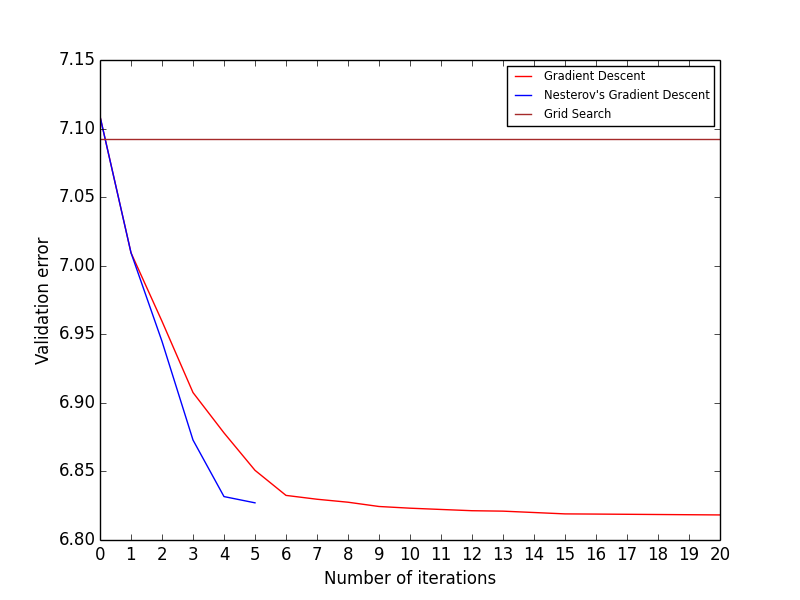
\includegraphics[width=70mm]{elasticnet_costpath_80_250_15.png}
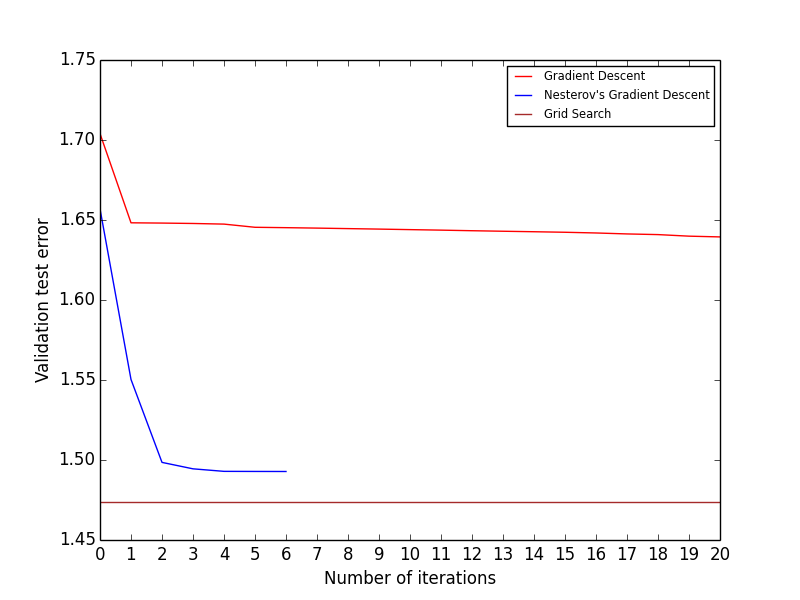
\includegraphics[width=70mm]{grouped_lasso_60_1500_3_150.png}
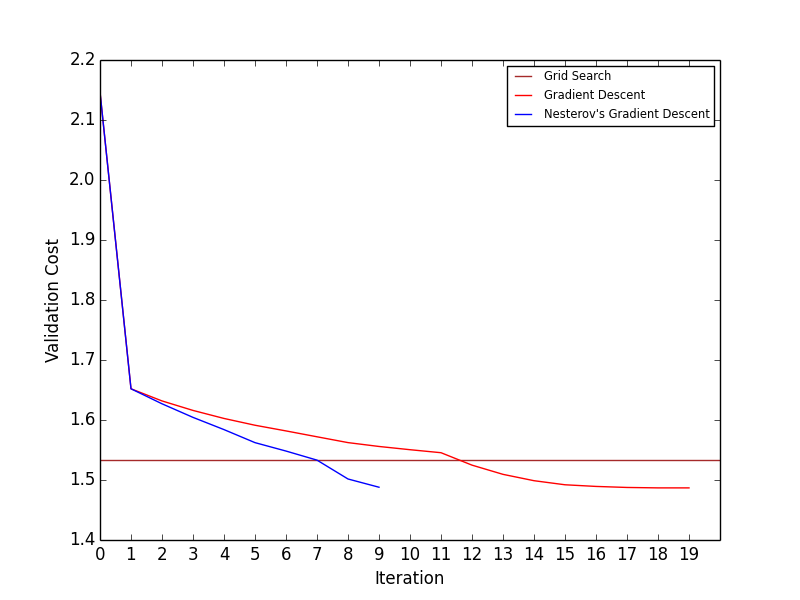
\includegraphics[width=70mm]{smooth_linear_simple_cost_path_1_100_20_6.png}
\caption{Validation error progression: Top Left - Elastic Net, Top Right - Grouped Lasso, Bottom Left - APLM}
\label{figure:costpath}
\end{figure}

\subsection{Discussion of results}

As shown in Table \ref{table:validation}, descent-based and grid-based joint optimization had the same performance in all three situations. The only major difference between the different implementations of joint optimization is in the runtimes. In every situation, gradient descent was over 40\% faster than the grid-based approach and Nesterov's subgradient descent was over 50\% faster.

Figure \ref{figure:costpath} shows example plots of how validation error decreases in the descent-based joint optimization procedures. The horizontal line in the plots are the lowest validation error achieved by grid-based joint optimization. In all three plots, Nesterov's gradient descent requires fewer iterations to minimize the validation loss.

\section{Results: regularizations with more than two penalties}

Our second simulation study is to show that descent-based joint optimization can effectively and efficiently solve regressions with more than two regularization parameters.

For each experiment, given a regularization method, we compared tuning the original two-parameter version using a grid-based approach to tuning the generalized, many-parameter version using gradient descent. In the sparse group lasso experiment, we tested an ``unpooled" version of sparse group lasso in which the the number of regularization parameters is linear in the number of covariate groups. In the APLM experiment, we tested having an additional ridge penalty for the linear regression coefficients. To compare the regularization methods, we measured the loss on the test sets. As shown later, since gradient descent for the generalized regression achieved a lower test set loss on average, we have shown that a descent-based approach for many-penalty regressions can produce better models than those from 2-penalty regressions.

The joint optimization problem formulations and gradient derivations for these generalized regularizations are given in the Appendix.

\subsection{Unpooled sparse group lasso}

In this experiment, we compared the effectiveness of applying gradient descent on an ``unpooled" variant of sparse group lasso to grid-based joint optimization on the regular sparse group lasso. In unpooled sparse group lasso, the group lasso penalty parameter $\lambda_1$ is replaced with an individual parameter for each covariate group:

\begin{equation}
\sum_{l=1}^m \lambda_1^{(k)} \lvert\lvert \beta^{(k)} \rvert \rvert_2
+ \lambda_2 \lvert\lvert \beta \rvert \rvert_1
\end{equation}
Hence, the number of regularization parameters increased from two to one plus the number of coefficient groups. This unpooled variant allows different thresholds to be used for setting coefficients and coefficient groups to zero, as opposed to the original sparse group lasso where the thresholds are shared. Potentially, this increased flexibility can produce more accurate models, especially when the covariate groups have very different distributions.

We ran three experiments, each with a different number of covariate groups $m$ and total covariates $p$. The simulation settings were similar to the first simulation study. Grid-based joint optimization for sparse group lasso was initialized with the same grid. Gradient descent for unpooled sparse group lasso was initialized with a lower set of values 1e-4, 1e-3, and 1e-2 to compensate for the fact that there are now $m + 1$ regularization parameters.

We measured three metrics to assess model performance: test error, $\beta$ error, which is defined as $\lvert \lvert \beta - \hat \beta \rvert \rvert_2 ^2$, and the percentage of nonzero coefficients correctly identified among all the true nonzero coefficients. As shown in Table \ref{table:unpooled}, unpooled sparse group lasso performed better according to all three metrics in all the experiments. Furthermore, gradient descent for unpooled sparse group lasso is faster than grid-based joint optimization for two-parameter sparse group lasso, even in the case with 151 regularization parameters.

\begin{table}
\begin{center}
\begin{tabular}{| l | l | l | l | l | }
\hline
\multicolumn{5}{|c|}{n=60, p=300, g=3, m=30}\\
\hline
 & $\beta$ Error & \% correct nonzero $\beta$ & Test Error & Runtime (sec) \\
\hline
Gridsearch (baseline) & 1.13 & 10.70 & 0.04 & 15.81 \\
\hline
Gradient Descent & 0.18 & 23.79 & 0.01 & 5.62 \\
\hline
\end{tabular}

%\vspace{5mm}
\begin{tabular}{| l | l | l | l | l | }
\hline
\multicolumn{5}{|c|}{n=60, p=1500, g=3, m=50}\\
\hline
 & $\beta$ Error & \% correct nonzero $\beta$ & Test Error & Runtime (sec) \\
\hline
Gridsearch (baseline) & 7.79 & 9.63 & 0.28 & 148.64 \\
\hline
Gradient Descent & 4.00 & 17.79 & 0.14 & 88.78 \\
\hline
\end{tabular}

%\vspace{5mm}
\begin{tabular}{| l | l | l | l | l | }
\hline
\multicolumn{5}{|c|}{n=60, p=1500, g=3, m=150}\\
\hline
 & $\beta$ Error & \% correct nonzero $\beta$ & Test Error & Runtime (sec) \\
\hline
Gridsearch (baseline) & 2.20 & 10.69 & 0.080 & 162.14 \\
\hline
Gradient Descent & 0.06 & 15.34 & 0.002 & 48.63 \\
\hline
\end{tabular}
\end{center}
\caption {Unpooled sparse group lasso}
\label{table:unpooled}
\end{table}

\subsection{Additive partial linear models with three regularization parameters}
In this example of joint optimization for APLMs, we experimented with a generalized version of the APLM regularization by using the elastic net instead of the lasso for the linear regression coefficients:
\begin{equation}
\lambda_1 \lvert\lvert \beta \rvert \rvert_1
+ \frac{1}{2} \lambda_2 \lvert\lvert \beta \rvert \rvert_2^2
+ \frac{1}{2} \lambda_3 \lvert\lvert D^{(2)} \theta \rvert \rvert_2^2
\end{equation}
We compared model fits from this three-parameter regularization tuned using gradient descent to those from the original two-parameter regularization tuned using a grid-based approach. Our hypothesis was that the elastic net penalty in this generalized regularization would produce more accurate models since it encourages both sparsity of representation and grouping among strongly correlated predictors.

We ran experiments on three nonlinear functions of varying levels of smoothness. The simulation settings were similar to before. The only difference was that gradient descent was initialized at the six points $\lambda_1 = \lambda_2 = \lambda_3 =10^i$ for $i=-4, ..., 1$.

Models were judged by their predictive accuracy. In addition, we used $\beta$ error, defined as $||\beta - \hat \beta||_2^2$, and $\theta$ error, defined as $|| g(z) - \theta ||_2^2$, to measure the error in the estimated linear and nonlinear components, respectively.

The results in Table \ref{ref:aplm} show that using three penalty terms in the criterion improved the models by all metrics. The biggest improvement was in the estimation of the linear regression components, which is expected since we added an penalty term for the linear coefficients. Somewhat surprisingly, the estimation of the nonlinear components also improved slightly, even though no penalty term was added for the nonlinear component. The runtime for tuning the three-parameter regularization was slightly longer than the grid-based version, but remained reasonable nonetheless. Most importantly, the increase in runtime is not exponential in the number of penalty parameters.

Figure \ref{fig:modelfits} shows example model fits from gradient descent and grid-based joint optimization. The plots confirm the hypothesis that the highly-correlated covariates are estimated better using the three-parameter regularization as opposed to the two-parameter one.


\begin{table}
\begin{center}
\begin{tabular}{| l | l | l | l | l | }
\hline
\multicolumn{5}{|c|}{$g(z) = 4z^3 - z^2 + 2z$}\\
\hline
 & $\beta$ Error & $\theta$ error & Test Error & Runtime (sec) \\
\hline
Gridsearch & 0.59 & 3.35 & 3.78 & 35.48 \\
\hline
Gradient Descent & 0.38 & 2.96 & 3.73 & 43.44 \\
\hline
\end{tabular}

%\vspace{5mm}
\begin{tabular}{| l | l | l | l | l | }
\hline
\multicolumn{5}{|c|}{$g(z) = \sin(5z) + \sin(15(z - 3))$}\\
\hline
 & $\beta$ Error & $\theta$ error & Test Error & Runtime (sec) \\
\hline
Gridsearch & 0.51 & 3.76 & 3.90 & 37.04 \\
\hline
Gradient Descent & 0.34 & 3.73 & 3.79 & 45.95 \\
\hline
\end{tabular}

%\vspace{5mm}
\begin{tabular}{| l | l | l | l | l | }
\hline
\multicolumn{5}{|c|}{$g(z) = (2-z)\sin(20z^4)$}\\
\hline
 & $\beta$ Error & $\theta$ error & Test Error & Runtime (sec) \\
\hline
Gridsearch & 0.58 & 4.91 & 4.13 & 40.75 \\
\hline
Gradient Descent & 0.41 & 4.85 & 4.08 & 54.63 \\
\hline
\end{tabular}
\end{center}
\caption {Additive Partial Linear Model}
\label{ref:aplm}
\end{table}

\begin{figure}
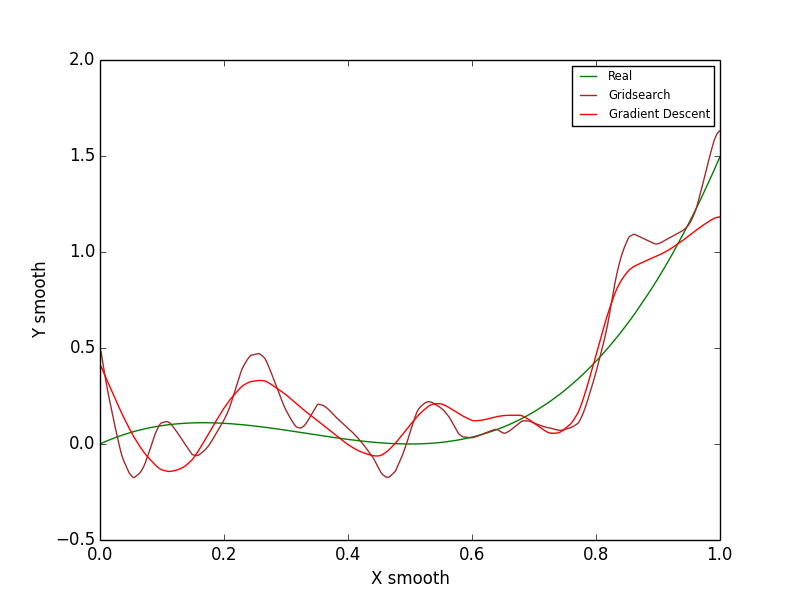
\includegraphics[height=40mm]{smooth_linear_thetas_2_100_20_6.png}
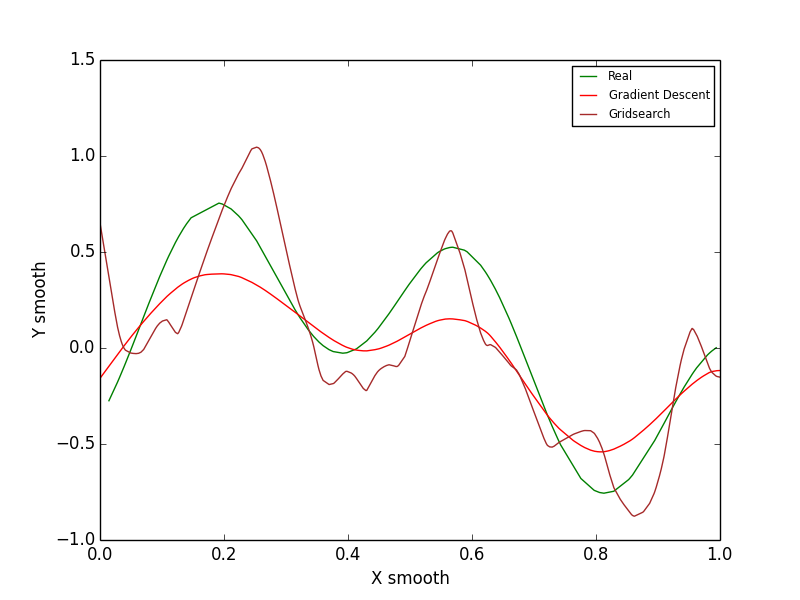
\includegraphics[height=40mm]{smooth_linear_thetas_0_100_20_6.png}
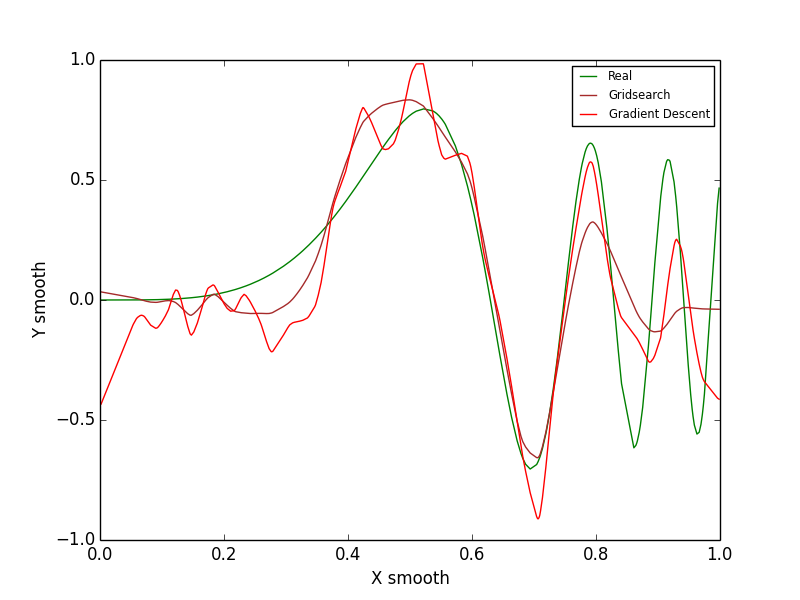
\includegraphics[height=40mm]{smooth_linear_thetas_1_100_20_6.png}
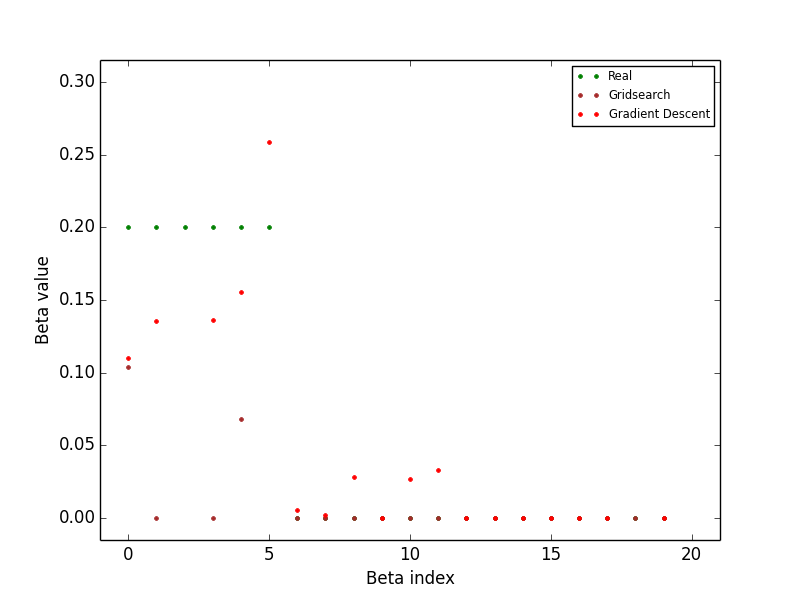
\includegraphics[height=40mm]{smooth_linear_beta_2_100_20_6.png}
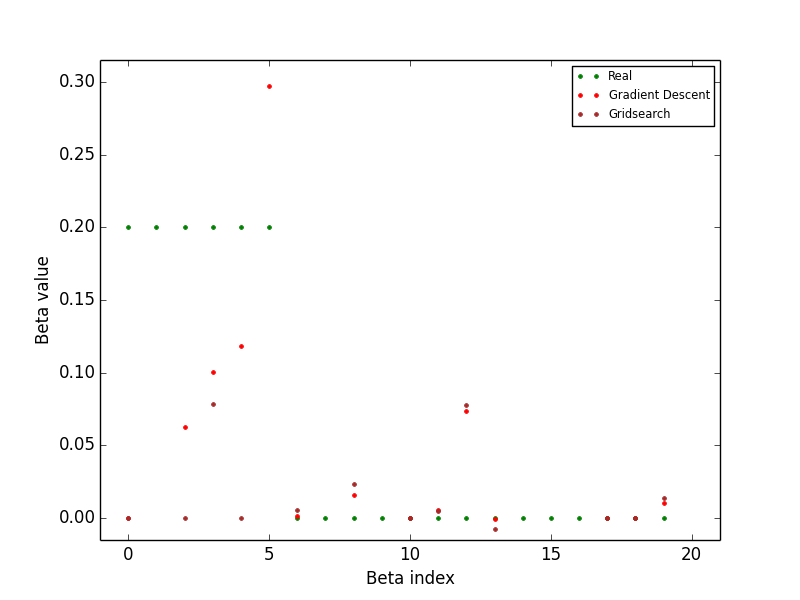
\includegraphics[height=40mm]{smooth_linear_beta_0_100_20_6.png}
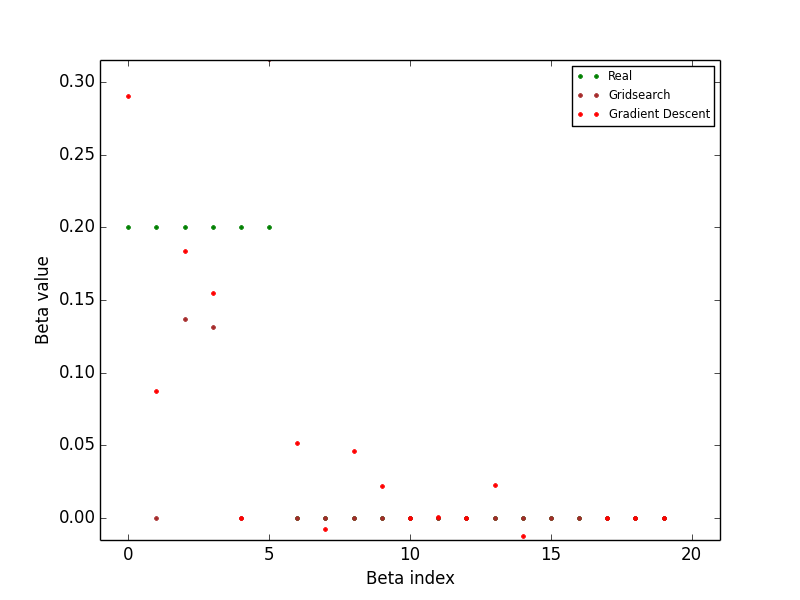
\includegraphics[height=40mm]{smooth_linear_beta_1_100_20_6.png}
\caption{Top: Example fits to the three smooth functions used in the experiments. The green line is the true function. Bottom: Example fits for the linear regression coefficients. The green is the true beta.}
\label{fig:modelfits}
\end{figure}

\section{Application to Real Data}
In this section, we discuss the performance and efficiency of joint optimization when applied to real data. We use un-pooled sparse group lasso as our example, since it can have the most number of penalty parameters among the regularization methods we previously mentioned. We compare this to sparse group lasso tuned using grid search.

We run regression to predict disease phenotype from gene expression data, as presented by Noah et. al. (2007). In this problem, the genes are grouped by gene pathways and we are interested in the pathways of interest and, from them, the driving genes.

Our dataset is from a colitis study of 127 total patients, 85 with colitis (59 crohn's patients + 26 ulcerative colitis patients) and 42 health controls (Burczynski 2006). Expression data was measured for 22,283 genes on affymetrix U133A microarrays. We grouped the genes according to the 326 C1 positional gene sets from MSigDb v5.0 (Subramanian 2005) and discarded the 2358 genes not found in the gene set. For each experiment, we randomly shuffled the data and used the first 50 observations for the training set and the remaining 77 for the test set. The experiment was repeated 10 times.

5-fold cross-validation was used to fit models. The penalty parameters in un-pooled sparse group lasso were all initialized at 0.5. For sparse group lasso, models were fit over a $5 \times 5$ grid of parameter values from 1e-4 to 5.

Perhaps the most important result is that joint optimization makes it possible to compare un-pooled sparse group lasso to sparse group lasso. Un-pooled sparse group lasso requires 327 regularization parameters for this problem, which is impossible to tune using grid search. Treating the problem as a continuous optimization problem not only makes it possible to tune many penalty parameters, but also makes the runtime comparable to grid search over two parameters, as seen in Table \ref{colitis}.

Un-pooled sparse group lasso and sparse group lasso achieve similar classification rates around 83\%. The primary difference is that un-pooled sparse group lasso finds solutions that are significantly more sparse than sparse group lasso -- on average, 9 genesets were identified, as opposed to 38. In addition, the number of genesets identified by un-pooled sparse group lasso has significantly lower variance. The number of genesets identified by sparse group lasso ranged from 2 to 73. The number of genesets identified by un-pooled sparse group lasso ranged from 8 to 12. Consistency is certainly an useful quality in regularization methods. These results suggest that un-pooling the penalty parameters in sparse group lasso can improve the regularization method. Further research is needed to determine if un-pooled sparse group lasso is a useful regularization method.

In this example, we have demonstrated that joint optimization is highly efficient at tuning parameters and can produce meaningful solutions to regression problems for real data.

\begin{table}
\begin{center}
\begin{tabular}{| l | l | l | l | l | }
\hline
 & \% correct  & Num. Genesets & Num. Genes & Runtime (sec) \\
\hline
SGL & 82.47 (0.7) & 38.4 (671.2) & 207.0 (22206.2) & 2722.4 \\
\hline
Unpooled SGL & 84.29 (0.3) & 8.9 (1.9) & 83.9 (664.5) & 2298.5 \\
\hline
\end{tabular}
\end{center}
\caption {Ulcerative Colitis Data: SGL = sparse group lasso, variance in parentheses}
\label{colitis}
\end{table}

\section{Discussion}
We proposed using joint optimization for tuning regularization parameters in both linear and nonlinear regressions. By treating the regression as an optimization problem over the regularization parameter space, joint optimization is highly scalable in the number of parameters. Through experiments on simulated data, we demonstrated that joint optimization is able to fit models with validation errors as low as grid search. We then increased the number of regularization parameters in traditional regularization methods and used joint optimization to fit even better models. During this exploration, we discovered that "unpooled" sparse group lasso has significantly better performance than the traditional sparse group lasso. Further research should be done to explore this new regularization method. Finally, we demonstrated that this method works well on real data.

This paper applied joint optimization to a number of criterions, but this method should be tested on more criterions to analyze its robustness. We also expect that by implementing joint optimization with more sophisticated optimization methods, we can expect significant gains in efficiency. Finally, it would be worthwhile to understand what types of situations are ill-suited for joint optimization and what is the maximum number of regularization parameters joint optimization can tune with reasonable computation time.

\section*{Appendix}

\subsection{Proof for Theorem \ref{thethrm}}

\begin{lemma}
Let the function $\hat f(\cdot)$ be defined as:
\begin{equation}
\hat f(\lambda) = \arg\min_f L(f, \lambda)
\end{equation}

For a given $\lambda_0$, suppose there exists a neighborhood around $\hat f(\lambda_0)$ such that for every $f$ in the neighborhood, $L(f, \lambda_0)$ is twice continuously differentiable with respect to $f$ and the hessian $Hess_f(L(f, \lambda_0))|_{\hat f(\lambda_0)}$ is nonsingular.
Then $\hat f(\cdot)$ is continuously differentiable in some neighborhood around $\lambda_0$.
\label{differentiablethrm}
\end{lemma}

\begin{proof}
Given that the loss function and penalty functions are differentiable, $\hat f(\lambda_0)$ is the point where the gradient of the function $L$ is zero:
\begin{equation}
\nabla_{f} L(f, \lambda_0) = 0
\end{equation}

Let $H(f, \lambda_0)$ denote the expression on the left hand side. From our assumptions, we know that $H(f, \lambda_0)$ is continuously differentiable with respect to $f$ in some neighborhood of $\hat f(\lambda_0)$ and the Jacobian matrix $D_f H(f, \lambda_0) |_{\hat f(\lambda_0)}$ is nonsingular. By the implicit function theorem, there exists a continuously differentiable function $\gamma$ such that for every $\lambda$ in some neighborhood around $\lambda_0$,
\begin{equation}
H(\gamma(\lambda), \lambda) = 0
\end{equation}
and
$\hat f(\lambda) = \gamma(\lambda)$.

\end{proof}

\begin{lemma}
Let $\hat f(\cdot)$ be defined as in lemma 1. For a given $\lambda_0$, suppose there exists a neighborhood around $f(\lambda_0)$ such that the regularity conditions from lemma 1 for $L(f, \lambda_0)$ only hold with respect to the active set of $f$. Furthermore, suppose there exists a neighborhood around $\lambda_0$ such that the non-active set of $\hat f(\cdot)$ is locally constant. Then $\hat f(\cdot)$ is continuously differentiable in some neighborhood around $\lambda_0$.
\label{activesetthrm}
\end{lemma}

\begin{proof}
By the KKT conditions, $\hat f(\lambda_0)$ is the point where the following subgradient condition is satisfied:

\begin{equation}
0 \in \partial_f L(f, \lambda_0)
\end{equation}

For the active set $\dot f$, the subgradient condition reduces to the gradient condition:

\begin{equation}
0 = \nabla_{\dot f} L(f, \lambda_0)
\label{gradientcondition}
\end{equation}

Applying Theorem \ref{differentiablethrm} to the gradient condition in (\ref{gradientcondition}), we know that the active set $\dot f(\cdot)$ is continuously differentiable for some neighborhood around $\lambda_0$. By our assumptions, the partial derivative of $\hat f(\cdot)$ with respect to the non-active set is zero in some neighborhood around $\lambda_0$. Combining the active and non-active sets, we have that $\hat f(\cdot)$ is continuously differentiable in some neighborhood around $\lambda_0$.

\end{proof}


\subsection{Elastic Net Gradient Derivations}
MATHS

\subsection{Sparse Group Lasso Derivations}

\subsubsection{Unpooled Sparse Group Lasso Derivations}
The gradient of the validation error with respect to the regularization parameters is:
\begin{equation}
\begin{array}{lcl}
\nabla_{\lambda_1^{(k)}} L(\boldsymbol y_V, X_V \hat \beta) &=& 
\frac{1}{n}
\Bigg (
X_V
(\frac{1}{n} X^T X + M_1 + M_2)^{-1}
\begin{bmatrix}
0 \\
\vdots \\
\frac{\hat\beta^{(l}}{||\hat\beta^{(l}||_2}\\
\vdots\\
0
\end{bmatrix}
\Bigg )^T
(\boldsymbol y_V - X_V \hat \beta)
 \\
\nabla_{\lambda_2} L(\boldsymbol y_V, X_V \hat \beta) &=&
\frac{1}{n}
\Bigg (
(\frac{1}{n} X^T X + M_1 + M_2)^{-1} sign(\hat \beta)
\Bigg )^T
(\boldsymbol y_V - X_V \hat \beta)
\\ 
\end{array}
\end{equation}

where $M_1$ is the block diagonal matrix with $l$ components 
$
\frac{\lambda_1^{(k)}}{|| \beta^{(k)}||_2^3}
\begin{bmatrix} 
\beta_1^{(k)} & 0 & \\
0 & \beta_2^{(k)} &  \\
 &  & \ddots \\
\end{bmatrix}
\begin{bmatrix}
\text{---} & \beta^{(k)T} & \text{---} \\
\text{---} & \beta^{(k)T} & \text{---} \\
\vdots
\end{bmatrix}
$ from top left to bottom right and $M_2$ is the diagonal matrix with $\frac{\lambda_1^{(k)}}{|| \beta^{(k)}||_2}$ from top left to bottom right.


\subsection{Additive Partial Linear Model Derivations}

\subsubsection{Additive Partial Linear Model Derivations: 3-penalties}

To perform joint optimization, we formulate the problem as follows:
\begin{multline}
\min_{\lambda_1, \lambda_2, \lambda_3} \frac{1}{2} \bigl\lvert\bigl\lvert \boldsymbol y_V - X_V\hat\beta - M_V \hat\theta \bigl\rvert\bigl\rvert^2_2 \\
\text{ where } \hat\beta, \hat\theta = \arg\min_{\beta, \theta} \frac{1}{2} \bigl\lvert\bigl\lvert y - X\beta - M_T \theta \bigl\rvert\bigl\rvert^2_2
+ \lambda_1 \lvert\lvert \beta \rvert \rvert_1
+ \frac{1}{2} \lambda_2 \lvert\lvert \beta \rvert \rvert_2^2
+ \frac{1}{2} \lambda_3 \lvert\lvert D^{(2)} \theta \rvert \rvert_2^2
\end{multline}
where $M_V \in \mathbb{R}^{|V| \times n}$ is the matrix such that $M_V X = X_V$ and $M_T \in \mathbb{R}^{|T| \times n}$ is the matrix such that $M_T X = X_T$ .

The gradients of the validation set error with respect to the regularization parameters are:
\begin{equation}
\nabla_{\lambda_i} L(\boldsymbol y_V, X_V \hat \beta + \hat \theta) = (X_V \frac{\partial \beta}{\partial \lambda_i} + M_V \frac{\partial \theta}{\partial \lambda_i})^T(\boldsymbol y_V - X_V \hat \beta - \hat \theta_V)
\end{equation}
where
\begin{equation}
\begin{array}{lcl}
\frac{\partial \beta}{\partial \lambda_1} &=& -(X_T^T X_T - X_T^T M_T(M_T^T M_T + \lambda_3 D^TD)^{-1} M_T^T X_T + \lambda_2 I)^{-1} sign(\hat \beta) \\
\frac{\partial \theta}{\partial \lambda_1} &=& -(M_T^T M_T + \lambda_3 D^T D)^{-1}  M_T^T X_T \frac{\partial \beta}{\partial \lambda_1}
\\
\frac{\partial \beta}{\partial \lambda_2} &=& -(X_T^T X_T - X_T^T M_T(M_T^T M_T + \lambda_3 D^TD)^{-1} M_T^T X_T + \lambda_2 I)^{-1} \hat \beta \\
\frac{\partial \theta}{\partial \lambda_2} &=& -(M_T^T M_T + \lambda_3 D^T D)^{-1}  M_T^T X_T \frac{\partial \beta}{\partial \lambda_2}
\\
\frac{\partial \theta}{\partial \lambda_3} &=& -(M_T^T M_T - M_T^T X_T (X_T^TX_T + \lambda_2 I)^{-1} X_T^T M_T + \lambda_3 D^TD)^{-1} D^TD \theta
\\
\frac{\partial \beta}{\partial \lambda_3} &=& - (X_T^TX_T + \lambda_2 I)^{-1} X_T^T M_T \frac{\partial \theta}{\partial \lambda_3} \\
\end{array}
\end{equation}

\section*{Acknowledgments}
BLAH


%\section*{References}
% Either type in your references using
% \begin{thebibliography}{}
% \bibitem{}
% Text
% \end{thebibliography}
%
% OR
%
% Compile your BiBTeX database using our plos2009.bst
% style file and paste the contents of your .bbl file
% here.
% 
\begin{thebibliography}{10}
\bibitem{bib1}
Lorem M, Ipsum VE (1990) Rank Correlation Methods. New York: Oxford University Press, 5th edition.

\end{thebibliography}

\end{document}

